

% ============================================================================
% 9.1 Resultados del an\'alisis distribucional
% ============================================================================
\section{An\'alisis distribucional de retornos}

El an\'alisis distribucional se aplic\'o a los 601 tickers del universo F5 sin pandemia, con 4\,207 ajustes param\'etricos. La Tabla~\ref{tab:stats_ticker} resume los estad\'isticos transversales y muestra dos rasgos centrales: la curtosis excedente es muy superior a la normalidad en casi todos los activos, con mediana 26,9 frente a 0 bajo normalidad, y la asimetr\'ia mediana es positiva (0,90), lo que sugiere colas derechas m\'as pesadas en el universo filtrado. El detalle completo del ajuste por distribuciones se presenta en el Anexo N°3.

\begin{table}[h]
\centering
\caption{Resumen transversal de estad\'isticos por ticker (universo F5 sin
pandemia).}
\label{tab:stats_ticker}
\scriptsize
\begin{tabular}{@{}lrrrr@{}}
\toprule
Variable & M\'in. & Mediana & Media & M\'ax. \\
\midrule
$n$ retornos & 2\,518 & 7\,949 & 8\,263 & 15\,400 \\
Media diaria & 0,011\% & 0,093\% & 0,102\% & 0,577\% \\
Vol. anualizada & 19,3\% & 36,5\% & 39,6\% & 214,9\% \\
VaR 5\% & $-$6,18\% & $-$3,04\% & $-$3,18\% & $-$1,63\% \\
CVaR 5\% & $-$10,93\% & $-$4,81\% & $-$5,09\% & $-$2,52\% \\
Asimetr\'ia & $-$8,40 & 0,90 & 3,44 & 99,13 \\
Curtosis exc. & 3,42 & 26,90 & 179,07 & 10\,151 \\
\bottomrule
\end{tabular}
\end{table}

La Tabla~\ref{tab:best_dist} confirma que la normal no es seleccionada como mejor distribuci\'on para ning\'un ticker, y las tres pruebas de normalidad rechazan la hip\'otesis nula al 5\% en los 601 casos. AIC y BIC coinciden en 532 tickers (88,5\%), aunque sus diferencias son informativas: AIC favorece Johnson SU por su flexibilidad para capturar asimetr\'ias, mientras BIC prefiere t-Student por capturar colas pesadas con mayor parsimonia.

\begin{table}[h]
\centering
\caption{Mejor familia distribucional seg\'un AIC y BIC.}
\label{tab:best_dist}
\scriptsize
\begin{tabular}{@{}lrrrr@{}}
\toprule
Distribuci\'on & AIC & \% & BIC & \% \\
\midrule
Johnson SU & 247 & 41,1 & 180 & 30,0 \\
t-Student & 179 & 29,8 & 241 & 40,1 \\
Normal generalizada & 174 & 29,0 & 176 & 29,3 \\
Laplace & 1 & 0,2 & 4 & 0,7 \\
Normal/log./skew-n. & 0 & 0,0 & 0 & 0,0 \\
\bottomrule
\end{tabular}
\end{table}

La prueba KS aproximada entrega valores-p mayores a 0,05 solo para el 36,5\% del universo bajo la mejor distribuci\'on. Por tanto, aunque las familias seleccionadas mejoran sustantivamente el supuesto normal, una distribuci\'on param\'etrica est\'atica no captura por completo dependencia temporal, volatilidad condicional ni cambios de r\'egimen. La implicancia directa es que la simulaci\'on Monte Carlo, al asumir retornos semanales normales, tiende a subestimar eventos extremos; por ello, sus resultados de riqueza terminal y tasa de retiro deben interpretarse como estimaciones bajo un r\'egimen ``normal'', no como predicciones robustas ante crisis.

% ============================================================================
% 9.2 Resultados Markowitz vs Benchmark
% ============================================================================
\section{Markowitz vs benchmark}

La Tabla~\ref{tab:markowitz_results} compara los KPIs del mejor portafolio Markowitz con el benchmark equiponderado en ambos escenarios de entrenamiento.

\begin{table*}[h]
\centering
\caption{Comparaci\'on Markowitz vs benchmark (horizonte h7\_f2, 601 activos,
rebalanceo semestral).}
\label{tab:markowitz_results}
\scriptsize
\begin{tabular}{@{}llrrrrrr@{}}
\toprule
Escenario & Portafolio & Ret. total & Ret. anual & Vol. anual & Drawdown &
CVaR 95\% & Sharpe \\
\midrule
Sin pandemia & Ideal de mercado & 76,5\% & 32,8\% & 12,3\% & $-$12,6\% &
1,7\% & 2,51 \\
Sin pandemia & Benchmark & 101,4\% & 41,9\% & 19,5\% & $-$21,9\% & 2,8\% &
2,05 \\
Con pandemia & Muy conservador & 54,5\% & 24,3\% & 11,0\% & $-$10,2\% &
1,5\% & 2,02 \\
Con pandemia & Benchmark & 101,4\% & 41,9\% & 19,5\% & $-$21,9\% & 2,8\% &
2,05 \\
\bottomrule
\end{tabular}
\end{table*}

Sin pandemia, el portafolio Ideal de mercado logra el mayor Sharpe del experimento (2,51), 0,46 puntos sobre el benchmark. Sin embargo, su retorno bruto es menor (76,5\% vs 101,4\%) y la mejora proviene de una volatilidad m\'as baja (12,3\% vs 19,5\%) y un drawdown m\'as contenido ($-$12,6\% vs $-$21,9\%). Con pandemia, el mejor Markowitz pasa a ser Muy conservador con Sharpe 2,02, pr\'acticamente igual al benchmark, lo que muestra que incluir 2020--2022 en la estimaci\'on de $\mu$ y $\Sigma$ reduce la capacidad del modelo para superar una regla simple.

\subsection{Impacto de la pandemia en Markowitz}

La Figura~\ref{fig:delta_pandemia} muestra el delta de Sharpe, definido como escenario con pandemia menos escenario sin pandemia. El deterioro es generalizado y aumenta con la agresividad del perfil: Ideal de mercado pierde 1,11 puntos, Muy arriesgado 0,86 y Arriesgado 0,57, mientras que M\'inima varianza ($-0,09$) y Benchmark ($-0,00$) son casi inmunes. Esto confirma que la sensibilidad a la pandemia crece con la dependencia del modelo respecto de retornos esperados, precisamente el componente m\'as afectado por el shock.

\begin{figure}[h]
    \centering
    \scriptsize
    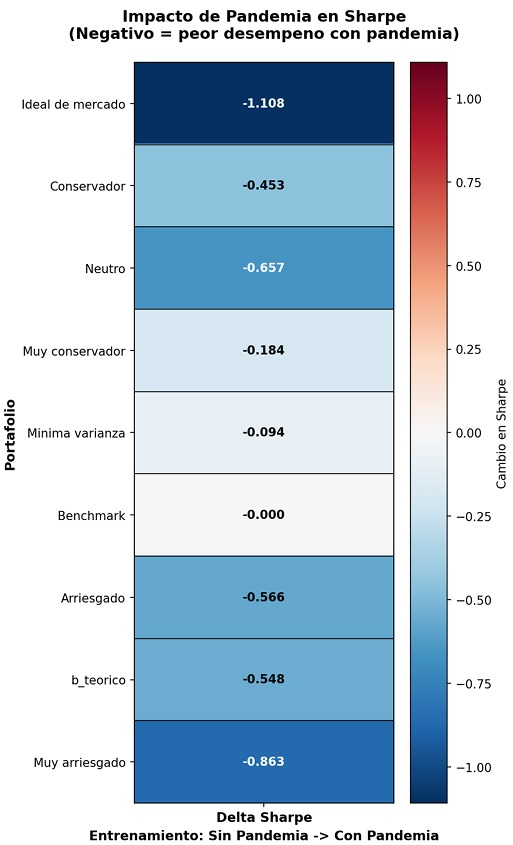
\includegraphics[width=0.55\textwidth]{figures/Impacto de la pandemia en Sharpe.jpeg}
    \caption{Delta de Sharpe por inclusi\'on de pandemia en el entrenamiento.}
    \label{fig:delta_pandemia}
\end{figure}

\subsection{Validaci\'on robusta}

La validaci\'on por ventanas m\'oviles confirma que horizontes m\'as largos de entrenamiento producen mejores Sharpe futuros: h7\_f2 alcanza 2,32 y el desempe\~no decrece monot\'onicamente hasta 1,35 en h2\_f7. Los 70 splits aleatorios tambi\'en identifican h7\_f2 como el horizonte \'optimo oficial para Markowitz.

% ============================================================================
% 9.3 Resultados Black-Litterman
% ============================================================================
\section{Black-Litterman}

La variante momentum top-20 a 6 meses domina en ambos escenarios, con Sharpe 2,46 sin pandemia y 2,38 con pandemia. Esta \textit{view} opera sobre un universo reducido, top 20 por capitalizaci\'on con 10 posiciones long y 10 short y 126 d\'ias de \textit{lookback}, combinando liquidez con se\~nal de momentum de mediano plazo. La \textit{view} de desempleo es la segunda m\'as competitiva y, con pandemia, obtiene Sharpe 2,36 en el perfil Arriesgado, 0,34 puntos sobre Markowitz puro. En cambio, momentum general, con 20 long y 20 short sobre los 601 activos, es la m\'as vol\'atil: sin pandemia llega a 2,38, pero con pandemia cae a 2,06, apenas igualando al benchmark.

\begin{table*}[h]
\centering
\caption{Mejor portafolio Black-Litterman por \textit{view} y escenario
(horizonte h7\_f2).}
\label{tab:bl_results}
\scriptsize
\begin{tabular}{@{}lllrrrrrr@{}}
\toprule
Escenario & View & Portafolio & Ret. total & Ret. anual & Vol. anual &
Drawdown & CVaR 95\% & Sharpe \\
\midrule
Sin pandemia & mom. top20 6m & Neutro & 72,3\% & 31,2\% & 11,9\% &
$-$12,9\% & 1,6\% & 2,46 \\
Sin pandemia & desempleo & Neutro & 63,1\% & 27,7\% & 10,5\% & $-$10,4\% &
1,4\% & 2,44 \\
Sin pandemia & momentum & Muy conserv. & 64,0\% & 28,1\% & 10,9\% &
$-$10,1\% & 1,5\% & 2,38 \\
Sin pandemia & mom. top20-b20 1y & Conservador & 63,1\% & 27,7\% & 10,9\% &
$-$10,7\% & 1,5\% & 2,35 \\
\midrule
Con pandemia & mom. top20 6m & Neutro & 69,5\% & 30,2\% & 11,9\% &
$-$11,7\% & 1,6\% & 2,38 \\
Con pandemia & desempleo & Arriesgado & 71,9\% & 31,1\% & 12,4\% &
$-$13,3\% & 1,7\% & 2,36 \\
Con pandemia & mom. top20-b20 1y & Neutro & 65,6\% & 28,7\% & 12,1\% &
$-$12,8\% & 1,7\% & 2,20 \\
Con pandemia & momentum & Conservador & 56,4\% & 25,0\% & 11,2\% &
$-$10,3\% & 1,5\% & 2,06 \\
\bottomrule
\end{tabular}
\end{table*}

La mejora de BL frente a Markowitz se concentra en el escenario con pandemia. La mayor ganancia aparece en BL desempleo/Arriesgado, con 1,19 puntos adicionales de Sharpe respecto del Markowitz equivalente. Sin pandemia, la brecha es menor porque Markowitz ya funciona bien con estimaciones hist\'oricas estables. As\'i, el principal valor de Black-Litterman es defensivo: ancla las estimaciones al equilibrio de mercado y reduce errores durante per\'iodos de estr\'es.

% ============================================================================
% 9.4 Resultados Monte Carlo P4
% ============================================================================
\section{Simulaci\'on Monte Carlo (P4)}

La Tabla~\ref{tab:p4_neutro} resume los promedios por t\'ecnica en el escenario proyectado neutro, promediando los cinco perfiles de riesgo.

\begin{table*}[h]
\centering
\caption{Promedios por t\'ecnica en escenario neutro (promedio de perfiles).}
\label{tab:p4_neutro}
\scriptsize
\begin{tabular}{@{}llrrrr@{}}
\toprule
T\'ecnica & View & Riqueza media & Retiro prom. & Utilidad empresa &
Prob. ganancia \\
\midrule
Equiponderado & No aplica & USD 4\,234 & 22,9\% & USD 234 & 77,1\% \\
BL Mom. Top20 6M & momentum\_top20\_6m & USD 4\,123 & 18,6\% & USD 253 &
81,3\% \\
BL Momentum & momentum & USD 3\,698 & 24,9\% & USD 223 & 74,6\% \\
BL Mom. Top20-B20 1Y & mom\_top20\_bottom20\_1y & USD 3\,213 & 19,9\% &
USD 174 & 79,8\% \\
BL Desempleo & desempleo & USD 3\,055 & 18,7\% & USD 160 & 81,2\% \\
Markowitz & Retornos hist\'oricos & USD 2\,970 & 21,3\% & USD 159 &
77,6\% \\
\bottomrule
\end{tabular}
\end{table*}

El Equiponderado lidera en riqueza bruta (USD~4\,234), pero mantiene una tasa de retiro alta (22,9\%). BL Momentum Top20 6M ofrece un equilibrio m\'as atractivo: riqueza similar (USD~4\,123), menor retiro (18,6\%), mayor utilidad para la empresa (USD~253) y la mayor probabilidad de ganancia (81,3\%). Markowitz queda \'ultimo en riqueza media (USD~2\,970), reforzando que, sin \textit{views}, no genera suficiente valor para el cliente promedio.

Para ordenar alternativas se usa el Score P4:
\begin{equation}
\text{Score}_{P4} =
E[\text{Riqueza terminal}]
+ E[\text{Utilidad empresa}]
- C_0 \cdot \text{Tasa de retiro}.
\end{equation}

El sistema recomienda la combinaci\'on con mayor Score P4, siempre que sus KPIs de riesgo sean consistentes con el perfil evaluado. La Tabla~\ref{tab:p4_ranking} presenta el top 5 del escenario neutro.

\begin{table*}[h]
\centering
\caption{Top 5 ranking P4 en escenario neutro.}
\label{tab:p4_ranking}
\scriptsize
\begin{tabular}{@{}clllrrrr@{}}
\toprule
Rank & Escenario & T\'ecnica & Perfil & Riqueza & Retiro & Utilidad &
Score P4 \\
\midrule
1 & Con pandemia & BL Mom. Top20 6M & Muy arriesgado & USD 8\,974 & 3,1\% &
USD 474 & 9\,417 \\
2 & Sin pandemia & BL Mom. Top20 6M & Muy arriesgado & USD 7\,753 & 2,0\% &
USD 419 & 8\,151 \\
3 & Con pandemia & BL Momentum & Muy arriesgado & USD 6\,436 & 14,6\% &
USD 335 & 6\,625 \\
4 & Sin pandemia & BL Momentum & Muy arriesgado & USD 5\,568 & 12,8\% &
USD 302 & 5\,831 \\
5 & Con pandemia & BL Mom. Top20 6M & Arriesgado & USD 5\,212 & 3,8\% &
USD 285 & 5\,486 \\
\bottomrule
\end{tabular}
\end{table*}

BL Momentum Top20 6M con perfil Muy arriesgado y datos de pandemia domina el ranking con Score 9\,417, combinando la mayor riqueza terminal (USD~8\,974), baja tasa de retiro para un perfil agresivo (3,1\%) y la mayor utilidad para la empresa (USD~474). Su ventaja se explica por la concentraci\'on de la se\~nal de momentum en activos l\'iquidos y estables, el \textit{lookback} de 126 d\'ias que captura tendencias de mediano plazo sin sobreajustar movimientos breves, y la alta tolerancia del perfil Muy arriesgado (40\%), que hace que $P_1$ casi nunca se active.

Los ganadores cambian seg\'un el escenario proyectado. En el favorable domina BL Momentum / Muy arriesgado / Con pandemia, con riqueza esperada de USD~12\,786; en el neutro gana BL Momentum Top20 6M / Muy arriesgado / Con pandemia, con USD~8\,974; y en el desfavorable lidera Equiponderado / Muy arriesgado / Sin pandemia, con USD~3\,759. Esta rotaci\'on es consistente: en condiciones favorables domina la estrategia m\'as agresiva sobre 601 activos, en condiciones desfavorables protege mejor el Equiponderado por no depender de estimaciones deterioradas, y en el escenario neutro sobresale BL Momentum Top20 6M por equilibrar momentum y estabilidad del prior de mercado.

% ============================================================================
% 9.5 An\'alisis integrado
% ============================================================================
\section{An\'alisis integrado}

La Tabla~\ref{tab:comparacion_final} sintetiza el mejor resultado de cada modelo por escenario.

\begin{table*}[h]
\centering
\caption{Comparaci\'on final: mejor portafolio por modelo y escenario.}
\label{tab:comparacion_final}
\scriptsize
\begin{tabular}{@{}llllrrr@{}}
\toprule
Escenario & Modelo & View & Portafolio & Ret. total & Sharpe & Drawdown \\
\midrule
Sin pandemia & Markowitz & Ret. hist\'oricos & Ideal de mercado & 76,5\% &
2,51 & $-$12,6\% \\
Sin pandemia & Black-Litterman & mom. top20 6m & Neutro & 72,3\% & 2,46 &
$-$12,9\% \\
Sin pandemia & Equiponderado & No aplica & Benchmark & 101,4\% & 2,05 &
$-$21,9\% \\
\midrule
Con pandemia & Black-Litterman & mom. top20 6m & Neutro & 69,5\% & 2,38 &
$-$11,7\% \\
Con pandemia & Black-Litterman & desempleo & Arriesgado & 71,9\% & 2,36 &
$-$13,3\% \\
Con pandemia & Equiponderado & No aplica & Benchmark & 101,4\% & 2,05 &
$-$21,9\% \\
Con pandemia & Markowitz & Ret. hist\'oricos & Muy conserv. & 54,5\% & 2,02 &
$-$10,2\% \\
\bottomrule
\end{tabular}
\end{table*}

En conjunto, los resultados muestran que sin pandemia Markowitz domina en Sharpe (2,51), aunque depende del portafolio Ideal de mercado y presenta \textit{overfitting}; Black-Litterman ofrece un Sharpe comparable (2,46) con menor dependencia de la estimaci\'on de $\mu$. Con pandemia, Black-Litterman lidera con Sharpe 2,38 y 2,36 seg\'un la \textit{view}, superando a Markowitz (2,02) por m\'as de 0,3 puntos gracias al prior de equilibrio. El benchmark equiponderado sigue siendo un competidor exigente en retorno bruto (101,4\%), pero su volatilidad (19,5\%) y drawdown ($-$21,9\%) lo hacen poco adecuado para perfiles conservadores, aunque su Sharpe de 2,05 establece un piso m\'inimo de desempe\~no. La validaci\'on robusta confirma que el Sharpe futuro cae al reducir la ventana de entrenamiento, y Monte Carlo identifica a BL Momentum Top20 6M como la mejor alternativa por Score P4, al combinar alta riqueza terminal, baja tasa de retiro y mayor utilidad para la empresa.

Las limitaciones principales se relacionan con supuestos simplificadores que conviene abordar en la siguiente etapa. La simulaci\'on Monte Carlo usa retornos normales pese al rechazo emp\'irico de normalidad; reemplazarlos por t-Student o Johnson SU producir\'ia colas m\'as realistas y posiblemente mayores tasas de retiro. Adem\'as, P4 mide p\'erdida respecto al capital inicial y no al m\'aximo alcanzado, por lo que usar \textit{drawdown} como gatillo de $P_1$ representar\'ia mejor la percepci\'on de p\'erdida del cliente. Tambi\'en falta sensibilizar $s = 20$, ya que cambios en este par\'ametro modificar\'ian las tasas de retiro y aceptaci\'on. Por \'ultimo, la \textit{view} de desempleo usa una tasa fija de 4\% frente a 5\% neutral en lugar de datos macroecon\'omicos observados; los escenarios proyectados son sim\'etricos ($\pm 0,5\sigma$), ignorando asimetr\'ia negativa; y la optimizaci\'on no incorpora costos de transacci\'on expl\'icitos, por lo que agregar restricciones o penalizaciones de rotaci\'on reducir\'ia el \textit{turnover} y alinear\'ia mejor la optimizaci\'on con la simulaci\'on.
